\documentclass[11pt,a4paper,twoside]{article}
\usepackage[utf8]{inputenc}
\usepackage[T1]{fontenc}
\usepackage{lmodern}
\usepackage[spanish,es-tabla,es-nodecimaldot]{babel}
\usepackage{microtype}
\usepackage[a4paper,inner=3cm,outer=2.5cm,top=2.6cm,bottom=2.6cm]{geometry}
\usepackage{amsmath,amssymb}
\usepackage{graphicx}
\usepackage{xcolor}
\usepackage{booktabs,tabularx,array,multirow,makecell}
\usepackage{enumitem}
\usepackage{caption,subcaption}
\usepackage{float}
\usepackage{fancyhdr}
\usepackage{titlesec}
\usepackage{setspace}
\usepackage{pdflscape}
\usepackage[hidelinks]{hyperref}
\makeatletter\renewcommand*\l@section{\@dottedtocline{1}{0em}{2.8em}}\makeatother

\definecolor{granate}{RGB}{138,0,0}
\definecolor{pizarra}{RGB}{43,58,85}
\newcommand{\porcompletar}[1]{\textcolor{red}{\textbf{[por completar: #1]}}}

\titleformat{\section}{\Large\bfseries\color{granate}}{\thesection.}{0.6em}{}
\titleformat{\subsection}{\large\bfseries\color{pizarra}}{\thesubsection}{0.6em}{}
\titleformat{\subsubsection}{\normalsize\bfseries\color{pizarra}}{\thesubsubsection}{0.6em}{}
\renewcommand{\thesection}{\Roman{section}}
\renewcommand{\thesubsection}{\thesection.\arabic{subsection}}
\captionsetup{font=small,labelfont=bf}
\setlist{itemsep=2pt,topsep=3pt}
\setstretch{1.08}

\pagestyle{fancy}
\fancyhf{}
\fancyhead[LE,RO]{\small\thepage}
\fancyhead[RE]{\small Presentación 1 · Proyecto Mecatrónico}
\fancyhead[LO]{\small Planificación de movimiento con aprendizaje por refuerzo}
\renewcommand{\headrulewidth}{0.4pt}

\newcommand{\E}{\mathbb{E}}
\newcommand{\dd}{\mathrm{d}}
\newcommand{\ind}{\mathbf{1}}

\begin{document}

\begin{titlepage}
\thispagestyle{empty}
\centering

\includegraphics[height=4.2cm]{img/logo_uni.png}\\[0.5cm]
{\Large\bfseries\textcolor{granate}{UNIVERSIDAD NACIONAL DE INGENIERÍA}}\\[3pt]
{\large Facultad de Ingeniería Mecánica}\\[2pt]
{\large Escuela Profesional de Ingeniería Mecatrónica}\\[1.2cm]
{\large Curso: \textbf{MT818 Proyecto Mecatrónico} · Sección A · 10.º ciclo · 2026-2}\\[0.5cm]
{\large Evaluación: \textbf{Presentación 1} (Informe técnico)}\\[1.4cm]
\rule{\linewidth}{1.2pt}\\[0.5cm]
{\LARGE\bfseries Planificación de movimiento y evasión de obstáculos mediante aprendizaje por refuerzo profundo para un manipulador industrial de 6 grados de libertad\par}
\vspace{0.4cm}
\rule{\linewidth}{1.2pt}\\[1.2cm]
{\large\textbf{Autores}}\\[4pt]
Caleb Camargo Saavedra \quad (20210011C)\\
Luis Leonardo Tupac Vásquez Cabrera \quad (\porcompletar{código})\\[0.9cm]
{\large\textbf{Profesor del curso}}\\[4pt]
Ing. José Oliden Martínez\\[0.3cm]
{\large\textbf{Asesor especializado}}\\[4pt]
Sin asesor especializado\\[1.2cm]
Lima, Perú · Octubre de 2026
\end{titlepage}

\tableofcontents
\clearpage

\section{Situación problemática y definición del problema}

\subsection{Situación problemática}

La manufactura moderna atraviesa un proceso sostenido de automatización. La Federación Internacional de Robótica (IFR) estimó que en 2024 se instalaron en el mundo unos 542\,000 robots industriales, casi el doble que una década antes, y que el parque operativo alcanzó 4\,664\,000 unidades, un 9\,\% más que el año anterior \cite{ifr2025}. Sin embargo, el crecimiento se concentra en grandes fábricas de producción en serie: Asia absorbió el 74\,\% de las instalaciones y China sola el 54\,\% \cite{ifr2025}. La IFR registraba apenas 48 robots industriales operativos en el Perú a finales de 2017, según datos citados en prensa especializada \cite{aduana2019}; no se encontró una cifra oficial más reciente, lo que ya es un indicio de la baja penetración.

En el país, el sector metalmecánico es un candidato natural a la automatización. El estudio del sector del Ministerio de la Producción (2024) lo describe como un conjunto de unas 74\,000 empresas que generan más de 350\,000 empleos y aportan más del 9\,\% del PBI manufacturero \cite{produce2025}. Son en su mayoría pequeñas empresas de producción de alta variedad y bajo volumen, es decir, lotes cortos de piezas distintas.

Ese perfil choca con la forma en que trabajan hoy los robots industriales. Un manipulador ejecuta trayectorias programadas punto a punto para una disposición concreta de máquinas, utillajes y piezas. Cuando la disposición cambia (un utillaje nuevo, un carro en otra posición, una pieza de otro tamaño), la trayectoria deja de ser válida: puede dejar de ser eficiente o producir una colisión, y hay que reprogramar o replanificar. En una celda de baja variedad ese costo se reparte entre miles de piezas; en una de alta variedad se paga en cada cambio. Los proveedores del sector estiman que la programación y la integración son una parte dominante del costo de ciclo de vida de una celda robotizada: un robot de USD 50\,000 puede acarrear USD 150\,000 o más de integración para una sola tarea \cite{fabricator}. Esas cifras son de fabricantes e integradores, no de estudios independientes, y se citan como orden de magnitud.

Las consecuencias de no resolver el problema son tres: (i) las pequeñas empresas descartan la automatización porque cada cambio de producto exige un ingeniero de integración; (ii) las celdas existentes quedan subutilizadas porque reprogramarlas detiene la producción; y (iii) se arriesgan colisiones costosas cuando se reutilizan trayectorias que ya no son válidas.

\subsection{Definición del problema}

\subsubsection{Problema general}

\emph{Limitada} capacidad de los manipuladores industriales de 6 grados de libertad para generar movimientos libres de colisión cuando cambia la disposición de obstáculos de la celda, pues dependen de trayectorias preprogramadas o de una replanificación completa de tiempo variable y costo de reconfiguración elevado.

\subsubsection{Problema ingenieril}

¿Qué consideraciones tecnológicas e ingenieriles de diseño mecatrónico y de diseño de software se tienen que tomar en cuenta a fin de desarrollar un planificador de movimiento reactivo, basado en aprendizaje por refuerzo profundo, para un manipulador de 6 GDL (DOBOT Magician E6), que satisfaga los requerimientos de evasión de obstáculos en celdas de manufactura reconfigurables, con el objetivo de reducir el costo de reconfiguración sin perder el desempeño de los planificadores clásicos?

\section{Estado del arte}

\subsection{Productos y soluciones existentes}

La Tabla~\ref{tab:productos} resume las soluciones comerciales y de código abierto que atacan, total o parcialmente, el problema. Todas calculan o ajustan trayectorias libres de colisión; ninguna es una política aprendida por refuerzo ni caracteriza cuánto se degrada ante geometrías no vistas.

\begin{table}[H]
\centering
\caption{Productos y soluciones existentes}
\label{tab:productos}
\small
\renewcommand{\arraystretch}{1.25}
\begin{tabularx}{\textwidth}{@{}>{\raggedright\arraybackslash}p{2.5cm}>{\raggedright\arraybackslash}X>{\raggedright\arraybackslash}X>{\raggedright\arraybackslash}p{2.6cm}@{}}
\toprule
\textbf{Producto} & \textbf{Ventajas} & \textbf{Desventajas y por qué no se usa} & \textbf{Precio} \\
\midrule
RapidPlan (Realtime Robotics) \cite{rapidplan} & Planes libres de colisión en milisegundos; mantiene trayectorias válidas ante cambios en vivo del piso de planta & Hardware propietario y subsistema de percepción aparte; licencia cerrada y costo por celda fuera del alcance de una pequeña empresa; no usa aprendizaje & Bajo cotización, no publicado \\
cuMotion en Isaac Manipulator (NVIDIA) \cite{cumotion} & Planificación acelerada por GPU en entornos congestionados; orientada a celdas que se reconfiguran & Exige GPU NVIDIA dedicada a bordo; es optimización en línea, no una política entrenada; no estudia generalización & SDK gratuito; GPU RTX aparte \\
RoboDK \cite{robodk} & Programación fuera de línea multimarca para más de mil robots; planificador PRM propio; accesible & Calcula rutas estáticas: los obstáculos son fijos en el modelo CAD, y cada cambio de utillaje obliga a replanificar y reexportar & Licencia educativa USD 145/año \cite{contexto}; profesional según lista \\
MoveIt 2 + OMPL \cite{moveit,ompl} & Código abierto; RRT-Connect, LazyPRM* y decenas de planificadores; estándar de facto en ROS & Tiempo de planificación variable (decenas de ms a segundos) y replanificación completa con cada cambio & Gratuito \\
\bottomrule
\end{tabularx}
\end{table}

Como referencia de costo del robot objetivo, el DOBOT Magician E6 (6 GDL, carga útil de 750\,g, alcance de 450\,mm, repetibilidad de $\pm$0.1\,mm) se vende en unos USD 6\,995 \cite{e6precio}. En este proyecto la unidad es prestada y no genera costo.

\subsection{Publicaciones científicas e ingenieriles}

Se revisaron cinco artículos, tres tesis y dos patentes. Aquí se describen los cuatro más relevantes; el resto figura en las referencias.

\paragraph{Mao et al. (2025) \cite{mao2025}.} Proponen evitar obstáculos dinámicos con un manipulador de 6 GDL mediante Soft Actor-Critic (SAC). La recompensa combina evitación de colisiones, autocolisión, alcance de la meta y suavidad; el estado incluye ángulos y velocidades articulares y puntos clave del cuerpo del robot. Se entrena en PyBullet con Gymnasium y Stable-Baselines3 y se valida en un UR5 real con cámara RealSense, con error de posición convergente y trayectorias suaves. Limitaciones: un solo robot, obstáculos simples, sin comparación con métodos clásicos ni evaluación de generalización. Es la referencia metodológica directa del proyecto, que conserva su formulación y añade esos elementos ausentes.

\paragraph{Fidalgo Astorquia et al. (2025) \cite{fidalgo2025}.} Es el antecedente más cercano. Construyen más de 100\,000 trayectorias libres de colisión con OMPL y comparan, con paridad de adaptadores ROS/MoveIt, los planificadores clásicos contra un agente SAC en un UR3e, con tiempo de planificación, tasa de éxito y suavidad. El agente logra mayor éxito y menor tiempo. Limitaciones: su entorno no contiene obstáculos (la observación de 14 valores solo incluye un indicador binario de colisión con el suelo o autocolisión, de modo que la tarea es alcanzar una pose en espacio libre), no evalúa generalización geométrica, y el agente se entrena con demostraciones del mismo método con el que luego se compara. Los propios autores reconocen que los planificadores clásicos conservan ventaja en adaptabilidad \emph{zero-shot}.

\paragraph{Jurgenson y Tamar (2019) \cite{jurgenson2019}.} Estudio fundacional de planificación neuronal por refuerzo que trata la generalización como pregunta central, y distingue variar inicio y meta sobre obstáculos fijos de variar la disposición de los obstáculos. La variante con demostraciones alcanza 0.93 de éxito en validación. Limitaciones: escenario de laboratorio, entrada visual de alta dimensión y sin comparación con OMPL en condiciones equivalentes.

\paragraph{Liu (2024) \cite{liu2024}.} Tesis de la Universidad de Toronto en la que una política PPO da órdenes de alto nivel a un controlador reactivo (Geometric Fabrics) que genera el movimiento. En un Franka Panda de 7 GDL alcanza 99.15\,\% de éxito y 0.64\,\% de colisión. Limitaciones: manipulador redundante, el aprendizaje no controla directamente las articulaciones y no reporta longitud de trayectoria ni distancia mínima.

La Tabla~\ref{tab:vacios} sintetiza el vacío que ocupa este proyecto: ningún trabajo reúne a la vez obstáculos, política aprendida aislada, comparación con clásicos en condiciones equivalentes y una medición explícita de generalización en un manipulador industrial de 6 GDL.

\begin{table}[H]
\centering
\caption{Mapa de vacíos del estado del arte (resumen de las fuentes revisadas)}
\label{tab:vacios}
\small
\begin{tabular}{@{}lccccc@{}}
\toprule
\textbf{Fuente} & \textbf{6 GDL} & \textbf{RL aislado} & \textbf{Obstáculos} & \textbf{vs. clásicos} & \textbf{Generaliz.} \\
\midrule
Mao et al. \cite{mao2025} & \checkmark & \checkmark & \checkmark & --- & --- \\
Fidalgo et al. \cite{fidalgo2025} & \checkmark & \checkmark & --- & \checkmark & --- \\
Jurgenson y Tamar \cite{jurgenson2019} & --- & \checkmark & \checkmark & --- & \checkmark \\
Liu \cite{liu2024} & \checkmark & --- & \checkmark & --- & --- \\
\textbf{Este proyecto} & \textbf{\checkmark} & \textbf{\checkmark} & \textbf{\checkmark} & \textbf{\checkmark} & \textbf{\checkmark} \\
\bottomrule
\end{tabular}
\end{table}

\section{Justificación}

\begin{itemize}
\item \textbf{Resuelve la situación problemática.} Una política que decide cada 30\,ms un incremento articular a partir de la geometría de los obstáculos no necesita que alguien reprograme la trayectoria cuando la celda cambia; solo exige que el cambio caiga dentro de lo que la política ha visto. El proyecto mide hasta dónde llega ese límite, que es lo que una pequeña empresa necesita saber antes de adoptar el enfoque.
\item \textbf{Barrera de costo.} Las soluciones comerciales exigen licencias cerradas o una GPU NVIDIA dedicada a bordo (Tabla~\ref{tab:productos}). La propuesta usa solo software de código abierto y una política que ocupa una fracción de milisegundo por paso en CPU (Sección~\ref{sec:avances}), con costo de software de S/\,0.
\item \textbf{Problemas de ingeniería que implica.} Software: modelo del robot fiable (el URDF oficial trae masas irreales de 0.94\,kg frente a 7.2\,kg, que hubo que corregir), formulación del proceso de decisión de Markov y de la recompensa, entrenamiento estable con varias semillas, módulo de distancia mínima validado contra FCL, equivalencia entre los motores de física de entrenamiento y de validación, y protocolo estadístico. Hardware e integración: diseño de la celda a escala de escritorio, singularidades de muñeca que justifican el espacio de acción, y presupuesto de latencia del lazo con el controlador del E6.
\item \textbf{Vacío científico.} El benchmark más riguroso frente a OMPL se hizo sin obstáculos en la escena \cite{fidalgo2025}; y ninguna fuente mide la generalización de la política en un manipulador industrial de 6 GDL (Tabla~\ref{tab:vacios}). Aportar esa medición con un protocolo reproducible es la novedad del trabajo.
\item \textbf{Normas y legislación.} El proyecto es de simulación: no pone a ninguna persona junto al robot, por lo que la colaboración humano-robot (ISO/TS 15066) queda fuera de alcance. La eventual puesta en una celda real deberá respetar ISO 10218-1 e ISO 10218-2 (seguridad de robots industriales) y la Ley N.º 29783 de Seguridad y Salud en el Trabajo. La verificación de colisiones se hace con el mismo evaluador para ambos métodos, lo que permite auditar la seguridad de cada trayectoria.
\item \textbf{Ambiental.} Simular y entrenar en computadora evita fabricar prototipos y consumir material en cada prueba; la política aprendida reutiliza el entrenamiento en lugar de recalcular cada vez.
\item \textbf{Inversión.} Todo el equipamiento ha sido prestado: no se ha realizado ningún gasto (Sección~\ref{sec:presupuesto}), por lo que la inversión es afrontable por los autores.
\end{itemize}

\section{Objetivos}

\subsection{Objetivo general}

Desarrollar y evaluar un planificador de movimiento reactivo, basado en aprendizaje por refuerzo profundo (SAC), que permita al manipulador DOBOT Magician E6 evitar obstáculos de forma y posición variables en una celda de manufactura, y compararlo con los planificadores clásicos de OMPL bajo condiciones equivalentes.

\subsection{Objetivos específicos}

\begin{table}[H]
\centering
\caption{Objetivos específicos con su indicador y su método de verificación}
\label{tab:oe}
\small
\renewcommand{\arraystretch}{1.3}
\begin{tabularx}{\textwidth}{@{}>{\raggedright\arraybackslash}p{0.7cm}>{\raggedright\arraybackslash}X>{\raggedright\arraybackslash}X>{\raggedright\arraybackslash}p{2.0cm}@{}}
\toprule
\textbf{N.º} & \textbf{Objetivo específico} & \textbf{Indicador de logro y verificación} & \textbf{Estado} \\
\midrule
1 & Modelar el Magician E6 y una celda de \emph{machine tending} a escala de escritorio como fuente única de geometría para PyBullet, MoveIt 2 y Gazebo. & Cinemática idéntica a la oficial y 91 pruebas automáticas aprobadas; los 8 escenarios se generan desde una biblioteca de componentes. & Logrado \\
2 & Definir un contrato de escenarios y las cinco métricas de desempeño. & Documento versionado con 100 escenas de evaluación fijas y 19 variantes; mismas definiciones para política y línea base. & Logrado \\
3 & Medir la línea base clásica (RRT-Connect y LazyPRM*) sobre las mismas escenas. & Al menos 100 escenas por planificador, con éxito, colisiones y tiempo reportados. & Logrado \\
4 & Entrenar una política SAC con tres semillas independientes. & Tres corridas de $10^6$ pasos con validación periódica y selección del mejor punto. & Logrado \\
5 & Validar la política contra la línea base y medir su generalización. & Prueba de Wilcoxon pareada por métrica ($\alpha=0.05$) en 100 escenas; éxito en los escenarios fuera de distribución. & En curso \\
6 & Diseñar la integración electrónica con el controlador del E6. & Diagrama de comunicación y presupuesto de latencia del lazo (lectura + inferencia + \texttt{ServoJ}) menor que 30\,ms. & Pendiente \\
\bottomrule
\end{tabularx}
\end{table}

\section{Descripción de la solución propuesta}

\subsection{Descripción}

\subsubsection{Diagrama de bloques pictórico}

\begin{landscape}
\begin{figure}[H]
\centering
\includegraphics[width=0.96\linewidth,height=0.72\textheight,keepaspectratio]{figuras/pictorico.pdf}
\caption{Diagrama de bloques pictórico del sistema.}
\label{fig:pictorico}
\end{figure}
\end{landscape}

\subsubsection{Funcionamiento}

\begin{enumerate}
\item El \textbf{contrato de escenarios} (archivo YAML versionado) fija el robot, la tarea (recoger una pieza en la bandeja y depositarla en la zona de carga del CNC), las cinco métricas y los criterios de terminación. La \textbf{biblioteca CAD} aporta los componentes de la celda.
\item El \textbf{generador de escenarios} compone cada escena: 100 de evaluación fijas, 50 de validación y escenas aleatorias de entrenamiento con forma, tamaño y posición del obstáculo muestreados.
\item El \textbf{entorno Gymnasium sobre PyBullet} simula el E6 con una transición cinemática de 30\,ms (el período de \texttt{ServoJ}). En cada paso entrega al agente una observación de 43 valores y una recompensa.
\item El \textbf{agente SAC} responde con un incremento articular $\Delta q\in[-0.05,0.05]^6$\,rad. Se entrena en la PC con GPU hasta $10^6$ pasos por semilla, con evaluaciones periódicas en escenas de validación.
\item Las mismas escenas se planifican con la \textbf{línea base} (MoveIt 2 + OMPL en ROS 2 Jazzy).
\item El \textbf{evaluador común} calcula las cinco métricas con el mismo código para ambos métodos y aplica la estadística pareada.
\item Como trabajo adicional fuera del alcance del curso, la política se ejecutaría en el E6 físico mediante \texttt{ServoJ}.
\end{enumerate}

\subsubsection{Dispositivos y componentes}

\begin{table}[H]
\centering
\caption{Componentes principales y justificación frente a alternativas}
\label{tab:componentes}
\small
\renewcommand{\arraystretch}{1.25}
\begin{tabularx}{\textwidth}{@{}>{\raggedright\arraybackslash}p{3.3cm}>{\raggedright\arraybackslash}X>{\raggedright\arraybackslash}X@{}}
\toprule
\textbf{Componente} & \textbf{Características} & \textbf{Por qué este y no otro} \\
\midrule
DOBOT Magician E6 & 6 GDL no redundante, alcance 450\,mm, carga 750\,g; publica URDF, mallas y MoveIt (licencia MIT); acepta posiciones articulares en línea (\texttt{ServoJ}, 33\,Hz) & Hay una unidad física en la universidad; la forma de su interfaz coincide con la acción $\Delta q$. Se descartó el UR5e (usado en las semanas 1 a 4) porque una política no se transfiere entre robots \\
PyBullet + Gymnasium + Stable-Baselines3 & Simulación rígida rápida (unas 1\,000 transiciones/s), entorno estándar y algoritmos SAC probados & Replica el stack de la referencia directa \cite{mao2025}; Isaac Sim se descartó por su curva de aprendizaje en un plazo de 15 semanas \\
ROS 2 Jazzy + MoveIt 2 + OMPL + Gazebo Harmonic & Planificadores de referencia (RRT-Connect, LazyPRM*) y simulador independiente & Es la práctica estándar del sector; mide la línea base con un motor distinto al de entrenamiento y obliga a verificar la equivalencia \\
SAC (actor-crítico de máxima entropía) & Fuera de política, acciones continuas, temperatura automática & Más eficiente en muestras que PPO y menos sensible a hiperparámetros que TD3 \\
PC de entrenamiento & 8 núcleos, 32\,GB, GPU GTX 1080 & Prestada; el entrenamiento con red pequeña y varias corridas en paralelo ocupa bien sus 8 núcleos \\
\bottomrule
\end{tabularx}
\end{table}

\subsubsection{Limitaciones de la solución}

\begin{itemize}
\item Percepción ideal: la posición, tamaño y orientación de los obstáculos se leen directamente del simulador. Los resultados son una cota superior del desempeño real; el supuesto se aplica por igual a la política y a la línea base.
\item Obstáculos estáticos durante cada episodio y primitivos geométricos (prisma, cilindro, esfera) o componentes de la biblioteca; no se modelan operarios humanos.
\item La comparación formal es en simulación. El despliegue en el E6 físico es trabajo adicional y no es objeto de estudio la transferencia \emph{sim-to-real}.
\item La política no ofrece garantías de completitud: en el escenario 8 (fuera de distribución) y en el paso estrecho, el planificador clásico sigue siendo la opción segura (Sección~\ref{sec:avances}).
\end{itemize}

\subsubsection{Resultados esperados}

Una política entrenada (con tres semillas o más) y una tabla comparativa con las cinco métricas frente a RRT-Connect y LazyPRM*; un criterio verificable sobre cuánta variación geométrica tolera la política antes de requerir replanificación clásica; y un repositorio reproducible con el modelo del E6, los escenarios, el entrenamiento y el evaluador. Se espera que la política responda con latencia menor y mayor holgura a los obstáculos que el planificador clásico, a costa de menor tasa de éxito en geometrías no vistas.

\subsection{Metodología de diseño e implementación}

\subsubsection{Descripción por etapas}

\paragraph{Etapa 1. Contrato experimental y métricas.} Definir la tarea, las tolerancias de terminación (5\,mm y 0.05\,rad), el límite de 300 pasos (9\,s), los ocho escenarios (espacio libre, obstáculo único, tres obstáculos, desplazado, redimensionado, forma mutada, paso estrecho y utillaje no visto) y las cinco métricas: tasa de éxito, colisiones, longitud de trayectoria, tiempo de ejecución y distancia mínima. \emph{Método}: diseño experimental con evaluación pareada.

\paragraph{Etapa 2. Modelo del robot y de la celda.} Obtener el URDF oficial del E6, corregir masas, límites y mallas de colisión con un generador (\texttt{gen\_modelo\_e6.py}), y diseñar la celda de \emph{machine tending} a escala de escritorio (mesa, centro CNC, bandeja, prensa, carro, pieza en tránsito). \emph{Métodos}: parámetros de Denavit-Hartenberg, cinemática directa e inversa, análisis de alcanzabilidad y de singularidades (manipulabilidad de Yoshikawa).

\paragraph{Etapa 3. Entorno y formulación del MDP.} Construir el entorno Gymnasium, el vector de observación de 43 valores, el espacio de acción $\Delta q$ y la recompensa. \emph{Métodos}: proceso de decisión de Markov, modelado de recompensa con potencial, distancia mínima eslabón-obstáculo validada contra FCL.

\paragraph{Etapa 4. Línea base clásica.} Configurar MoveIt 2 y OMPL (RRT-Connect y LazyPRM*), un tiempo máximo de 5\,s y el mismo perfil de velocidad que la política, y medir las 100 escenas con las mismas métricas.

\paragraph{Etapa 5. Entrenamiento SAC.} Entrenar con tres semillas ($10^6$ pasos, cuatro entornos en paralelo), con validación cada 50\,000 pasos y selección del mejor punto. Explorar mejoras de muestreo de los obstáculos y de la recompensa (\texttt{sac\_v2}).

\paragraph{Etapa 6. Evaluación, generalización y validación estadística.} Evaluar cada modelo una sola vez en las 100 escenas de evaluación y en las 19 variantes del contrato; comparar con la línea base mediante la prueba de rangos con signo de Wilcoxon y analizar dónde falla la política (por tamaño, forma y posición).

\paragraph{Etapa 7. Integración con el E6: diseño electrónico.} Diseñar la arquitectura de control (TCP/IP, lazo \texttt{ServoJ} de 33\,Hz), la unidad de cómputo, el sensado de la pose de los obstáculos, la cadena de seguridad y el presupuesto de latencia.

\paragraph{Etapa 8 (adicional).} Ejecutar la política en el E6 físico, fuera del alcance obligatorio del curso.

\subsubsection{Diagrama de bloques de la metodología}

\begin{figure}[H]
\centering
\includegraphics[width=\textwidth]{figuras/metodologia.pdf}
\caption{Diagrama de bloques de las etapas de desarrollo.}
\label{fig:metodologia}
\end{figure}

\section{Marco teórico}

\subsection{Proceso de decisión de Markov y aprendizaje por refuerzo}

El problema se formula como un proceso de decisión de Markov $(\mathcal{S},\mathcal{A},P,r,\gamma)$. En cada instante $t$ el agente observa $s_t$, elige $a_t\sim\pi(\cdot\mid s_t)$ y recibe $r_t$. El objetivo es hallar la política que maximiza el retorno descontado esperado \cite{sutton2018}:
\begin{equation}
J(\pi)=\E_{\pi}\!\left[\sum_{t=0}^{\infty}\gamma^{t}\,r(s_t,a_t)\right],\qquad \gamma=0.99 .
\end{equation}

\paragraph{Estado y acción en este proyecto.} La observación tiene 43 valores: posiciones articulares normalizadas (6), el incremento anterior (6), el error de posición del efector a la meta (3), el error de orientación como cuaternión (4), y para cada uno de los seis eslabones la distancia mínima a un objeto (6) y la dirección unitaria hacia él (18). La acción es $a\in[-1,1]^6$, que se traduce a $\Delta q = 0.05\,a$\,rad y a una transición cinemática $q_{t+1}=\mathrm{clip}(q_t+\Delta q)$ dentro de los límites articulares.

\paragraph{Recompensa.} Combina progreso hacia la meta, orientación, un potencial de precisión, castigo por proximidad, suavidad y tiempo, con premio al éxito y castigo a la colisión:
\begin{equation}
r_t = 10\,\frac{\Delta d}{L}+5\,\Delta\theta+10\,\Delta\Phi-w_p-w_s-0.01-10\,\ind_{\mathrm{col}}+10\,\ind_{\mathrm{éxito}},
\end{equation}
con $\Phi(d,\theta)=e^{-d/0.02}\,e^{-\theta/0.10}$, $d$ el error de posición (m), $\theta$ el error angular (rad) y $L=0.427$\,m la longitud de la tarea. $\Delta d$ y $\Delta\theta$ son las reducciones de $d$ y de $\theta$ respecto al paso anterior, y $\Delta\Phi=\Phi_t-\Phi_{t-1}$ (conformación por potencial). El castigo por proximidad es $w_p=\max\!\bigl(0,\,1-d_{\min}/0.02\bigr)$, con $d_{\min}$ la distancia mínima a cualquier objeto (m), y el de suavidad es $w_s=0.05\,\lVert(\Delta q_t-\Delta q_{t-1})/0.05\rVert^2/6$.

\subsection{Soft Actor-Critic (SAC)}

SAC \cite{haarnoja2018} maximiza el retorno más la entropía de la política, lo que favorece la exploración y evita óptimos locales:
\begin{equation}
J(\pi)=\sum_{t}\E_{(s_t,a_t)\sim\rho_\pi}\bigl[r(s_t,a_t)+\alpha\,\mathcal{H}(\pi(\cdot\mid s_t))\bigr].
\end{equation}
Usa dos críticos $Q_{\theta_1},Q_{\theta_2}$ y sus redes objetivo $\bar\theta_i$. El valor objetivo toma el mínimo de los dos para evitar sobreestimación:
\begin{equation}
y=r+\gamma(1-d)\Bigl(\min_{i}Q_{\bar\theta_i}(s',a')-\alpha\log\pi_\phi(a'\mid s')\Bigr),\qquad a'\sim\pi_\phi(\cdot\mid s').
\end{equation}
Cada crítico se entrena minimizando el error cuadrático, y el actor, con la técnica de reparametrización $a=\tanh(\mu_\phi+\sigma_\phi\odot\varepsilon)$, $\varepsilon\sim\mathcal{N}(0,I)$:
\begin{align}
J_Q(\theta_i)&=\E\bigl[(Q_{\theta_i}(s,a)-y)^2\bigr],\\
J_\pi(\phi)&=\E\bigl[\alpha\log\pi_\phi(a\mid s)-\min_i Q_{\theta_i}(s,a)\bigr].
\end{align}
La temperatura $\alpha$ se ajusta automáticamente hacia una entropía objetivo $\bar{\mathcal{H}}=-\dim(\mathcal{A})=-6$ \cite{haarnoja2018b}, y las redes objetivo se actualizan de forma suave:
\begin{equation}
J(\alpha)=\E\bigl[-\alpha\bigl(\log\pi_\phi(a\mid s)+\bar{\mathcal{H}}\bigr)\bigr],\qquad
\bar\theta_i\leftarrow\tau\theta_i+(1-\tau)\bar\theta_i,\ \ \tau=0.005 .
\end{equation}
Hiperparámetros: tasa de aprendizaje $3\times10^{-4}$, lote de 256, búfer de $10^6$ transiciones y redes de $256\times256$ neuronas. Se usa Stable-Baselines3 \cite{sb3}.

\subsection{Cinemática y análisis del manipulador}

La cinemática directa del E6 se obtiene con los parámetros de Denavit-Hartenberg \cite{siciliano2009}: $T_0^6(q)=\prod_{i=1}^{6}A_i(\theta_i)$, con $A_i$ la matriz homogénea de cada eslabón. El jacobiano $J(q)\in\mathbb{R}^{6\times6}$ relaciona velocidades articulares y del efector, y la manipulabilidad de Yoshikawa $w(q)=\lvert\det J(q)\rvert$ se anula en las singularidades. En el E6 la singularidad de muñeca (J5 próxima a 0) justifica que la acción sea un incremento articular acotado y no una orden cartesiana, que cruzaría esa configuración con velocidades articulares no acotadas.

\begin{figure}[H]
\centering
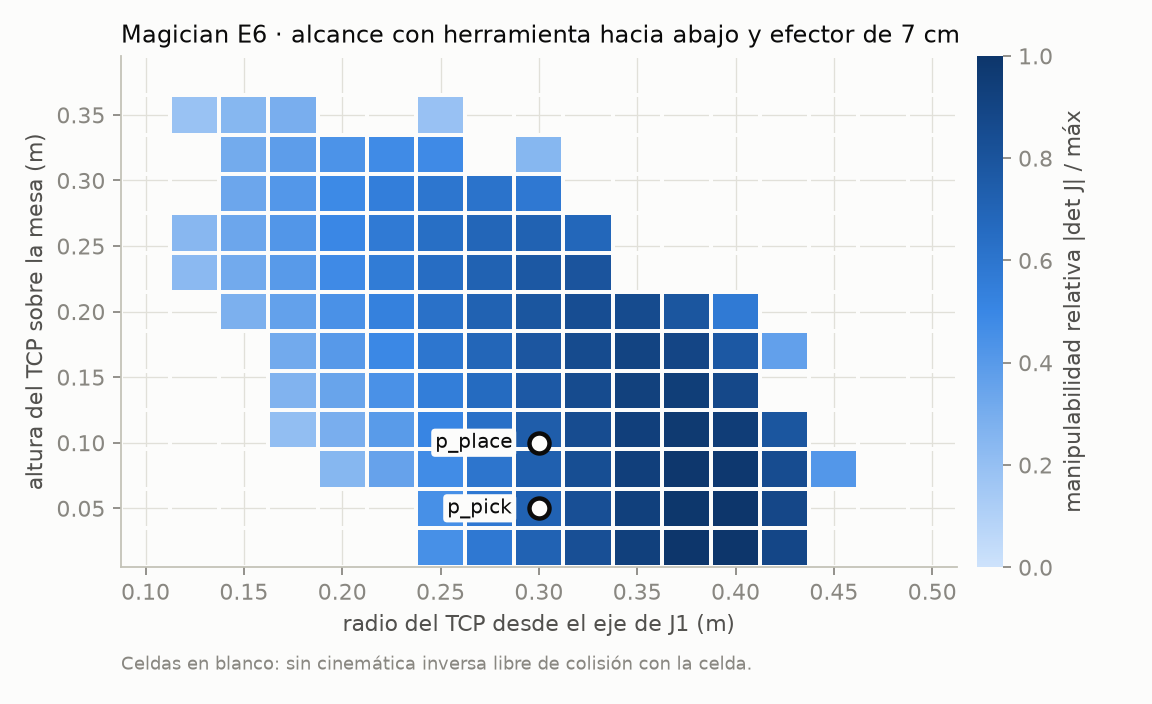
\includegraphics[width=0.78\textwidth]{img/alcanzabilidad_e6.png}
\caption{Alcanzabilidad del E6 con herramienta hacia abajo; 105 de 221 puntos del plano de trabajo tienen cinemática inversa libre de colisión. Las poses de recogida y de depósito están en la zona de mayor manipulabilidad.}
\label{fig:alcance}
\end{figure}

\subsection{Planificación clásica por muestreo}

\emph{RRT-Connect} \cite{kuffner2000} hace crecer dos árboles de configuraciones libres, desde el inicio y desde la meta, y los conecta; es rápido, probabilísticamente completo y entrega trayectorias quebradas. \emph{LazyPRM*} \cite{bohlin2000} construye un grafo de configuraciones y pospone las verificaciones de colisión hasta que una ruta candidata las necesita, y con el criterio asintóticamente óptimo de PRM* \cite{karaman2011} converge a rutas más cortas con más tiempo. Ambos se ejecutan en OMPL \cite{ompl} desde MoveIt 2 \cite{moveit}. La verificación de colisiones usa la biblioteca FCL \cite{fcl}.

\subsection{Métricas y estadística de comparación}

Para $N$ escenas, con $\ind_i$ la indicadora de éxito (meta alcanzada dentro de tolerancia, sin colisiones y a tiempo):
\begin{equation}
\text{M1}=\frac1N\sum_{i=1}^{N}\ind_i,
\end{equation}
y M2 es el número de entradas en contacto por par (eslabón, objeto). Las longitudes y la distancia mínima son
\begin{align}
L_{\mathrm{cart}}&=\sum_{k}\lVert p(t_{k+1})-p(t_k)\rVert_2,\qquad
L_{\mathrm{art}}=\sum_{k}\lVert q(t_{k+1})-q(t_k)\rVert_2,\\
d_{\min}&=\min_{k}\ \min_{j}\ d\bigl(\text{eslabón}_j(t_k),\text{obstáculos}\bigr).
\end{align}
M4 es el tiempo de cómputo (suma de las inferencias de la política en el episodio, o el tiempo de planificación de OMPL) y el tiempo de ejecución de la trayectoria. Como ambos métodos resuelven las mismas escenas, se comparan por pares con la \emph{prueba de rangos con signo de Wilcoxon} \cite{wilcoxon1945}, con $\alpha=0.05$ y sin supuesto de normalidad.

\section{Aplicaciones y usuarios potenciales}

\paragraph{Aplicaciones directas.} Abastecimiento de máquinas CNC (\emph{machine tending}) en celdas flexibles; paletizado y manipulación de piezas con utillajes que cambian; reposicionamiento de brazos entre estaciones compartidas.

\paragraph{Aplicaciones indirectas.} Línea base y marco de evaluación reutilizable para comparar cualquier nuevo planificador de manipuladores; material docente de la escuela (el entorno, los escenarios y el evaluador son reproducibles); punto de partida para estudios con percepción real o con obstáculos dinámicos.

\paragraph{Usuarios potenciales.} Pequeñas y medianas empresas metalmecánicas con alta variedad de productos, integradores de robots, laboratorios y escuelas de ingeniería con brazos de escritorio.

\section{Viabilidad}

\paragraph{Técnica.} El grupo cuenta con los conocimientos de cinemática, control, programación y aprendizaje automático necesarios; ya funcionan el modelo del E6, el entorno de simulación, la línea base y tres entrenamientos completos. La universidad presta el E6 y una PC con GPU. Las herramientas son de código abierto y de fácil acceso. El proyecto es técnicamente posible: la política alcanza hasta 87\,\% de éxito en 100 escenas, lo que muestra que el enfoque funciona aunque todavía no iguala a la línea base.

\paragraph{Económica.} Costo de inversión hasta la fecha: S/\,0 (Sección~\ref{sec:presupuesto}). La principal ventaja frente al mercado es la ausencia de licencias y de GPU dedicada a bordo. El mercado potencial es el sector metalmecánico peruano (unas 74\,000 empresas \cite{produce2025}), aunque este proyecto no es un producto comercial sino un estudio que informa cuándo adoptar esta técnica.

\paragraph{Social.} Beneficia a las pequeñas empresas al reducir el costo de automatizar producción variable. No pone en riesgo a personas porque es solo de simulación.

\paragraph{Operativa.} Requiere una PC con GPU para entrenar (unas 4 h por corrida con cuatro en paralelo) y un procesador convencional para la inferencia. Las ampliaciones futuras son: percepción real, obstáculos dinámicos, despliegue en el E6 y comparación con otros algoritmos (PPO, TD3).

\paragraph{Alternativas consideradas.} Entrenar y evaluar todo dentro de ROS 2/Gazebo (se descartó por velocidad); Isaac Sim (curva de aprendizaje); mantener el UR5e (no hay unidad física); aprendizaje con demostraciones de OMPL (se descartó para no comprometer la independencia de la comparación).

\section{Cronograma semanal de desarrollo del proyecto}

La Figura~\ref{fig:crono} muestra el cronograma de las 16 semanas. En verde lo realizado, en ámbar lo que está en curso y en gris lo pendiente; la línea granate marca la semana actual (semana 9).

\begin{landscape}
\begin{figure}[H]
\centering
\includegraphics[width=0.96\linewidth,height=0.72\textheight,keepaspectratio]{figuras/cronograma.pdf}
\caption{Cronograma semanal con lo realizado, lo en curso y lo pendiente.}
\label{fig:crono}
\end{figure}
\end{landscape}

\begin{table}[H]
\centering
\caption{Cronograma por actividades del curso}
\small
\renewcommand{\arraystretch}{1.2}
\begin{tabularx}{\textwidth}{@{}>{\raggedright\arraybackslash}p{4.0cm}>{\raggedright\arraybackslash}X>{\centering\arraybackslash}p{1.4cm}@{}}
\toprule
\textbf{Actividad} & \textbf{Aspectos considerados} & \textbf{Semana} \\
\midrule
Presentación del curso y tema & Temas actuales; aprobación del tema con el docente & 1--3 \\
Formación de grupo y definición de objetivos & Grupo de dos; objetivo general y específicos con indicador & 3--5 \\
Primera revisión de avance (\textbf{Presentación 1}) & Estado del arte, justificación, solución propuesta, avances de simulación y línea base & 9 \\
Entrenamiento y evaluación & Núcleo de 3 semillas hecho; mejoras de muestreo y recompensa & 8--11 \\
Segunda revisión de avance (Presentación 2) & Cálculos, simulación, video de 5 minutos & 11--12 \\
Análisis, demostración e informe & Estadística completa, escenario 8, demo en vivo e informe & 12--15 \\
Presentación final & Informe, exposición y demostración & 15--16 \\
\bottomrule
\end{tabularx}
\end{table}

\section{Presupuesto económico del proyecto}
\label{sec:presupuesto}

Todo lo que se ha usado ha sido prestado por la universidad o por el profesor y se considera de costo cero, según la regla del curso. El único gasto previsto es la impresión de los entregables, cuyo monto es una estimación por confirmar.

\begin{table}[H]
\centering
\caption{Presupuesto del proyecto}
\small
\renewcommand{\arraystretch}{1.25}
\begin{tabularx}{\textwidth}{@{}>{\raggedright\arraybackslash}p{2.6cm}>{\raggedright\arraybackslash}X>{\centering\arraybackslash}p{0.8cm}>{\raggedleft\arraybackslash}p{1.5cm}>{\raggedleft\arraybackslash}p{1.5cm}>{\raggedright\arraybackslash}p{2.9cm}@{}}
\toprule
\textbf{Nombre} & \textbf{Uso} & \textbf{Cant.} & \textbf{Costo unit. (S/)} & \textbf{Total (S/)} & \textbf{Comentarios} \\
\midrule
DOBOT Magician E6 & Robot objetivo; modelo y, como trabajo adicional, pruebas reales & 1 & 0.00 & 0.00 & Prestado por el profesor; referencia de mercado USD 6\,995 \\
PC de entrenamiento (GTX 1080, 8 núcleos, 32\,GB) & Entrenamiento de las políticas SAC & 1 & 0.00 & 0.00 & Prestada \\
Computadora portátil & Desarrollo, simulación y evaluación & 1 & 0.00 & 0.00 & Equipo ya disponible \\
Software (ROS 2, MoveIt 2, OMPL, Gazebo, PyBullet, PyTorch, Stable-Baselines3) & Simulación, línea base y entrenamiento & --- & 0.00 & 0.00 & Código abierto \\
Impresión de informe y diapositivas & Entregables de la Presentación 1 (doble cara) & 1 & 20.00 & 20.00 & Estimado, por confirmar \\
Mano de obra & Dos estudiantes del curso & 2 & 0.00 & 0.00 & No monetizada \\
\midrule
\multicolumn{4}{@{}r}{\textbf{TOTAL}} & \textbf{20.00} & \\
\bottomrule
\end{tabularx}
\end{table}

\section{Descripción del producto final de Proyecto Mecatrónico}

\subsection{Diagrama pictórico con lo que se implementa}

\begin{landscape}
\begin{figure}[H]
\centering
\includegraphics[width=0.96\linewidth,height=0.72\textheight,keepaspectratio]{figuras/pictorico_resaltado.pdf}
\caption{Diagrama pictórico: en granate lo que se implementa en el curso; en gris, lo que queda como trabajo adicional.}
\end{figure}
\end{landscape}

\subsection{Diagrama metodológico con las etapas a desarrollar}

\begin{figure}[H]
\centering
\includegraphics[width=\textwidth]{figuras/metodologia_resaltada.pdf}
\caption{Diagrama metodológico: etapas 1 a 7 se realizan en el curso; la etapa 8 es adicional.}
\end{figure}

\subsection{Descripción}

Al final del curso se entregará: (i) el modelo corregido del Magician E6 y la celda de escritorio en PyBullet, MoveIt 2 y Gazebo; (ii) el entorno Gymnasium con el MDP documentado; (iii) el banco de pruebas con la línea base clásica; (iv) políticas SAC entrenadas con al menos tres semillas, con la evaluación estadística frente a la línea base y el análisis de generalización; (v) una demostración en vivo en simulación con un tablero comparativo de las cinco métricas; (vi) el diseño de la integración electrónica con el controlador del E6; y (vii) el informe final y un repositorio reproducible.

\subsection{Avances alcanzados y validación de resultados}
\label{sec:avances}

Este apartado reúne lo ya medido, como evidencia de la viabilidad (Art.~8 y 10 del reglamento). Todas las cifras proceden de los archivos de resultados del repositorio.

\subsubsection{Entorno y escenarios}

\begin{figure}[H]
\centering
\begin{subfigure}{0.48\textwidth}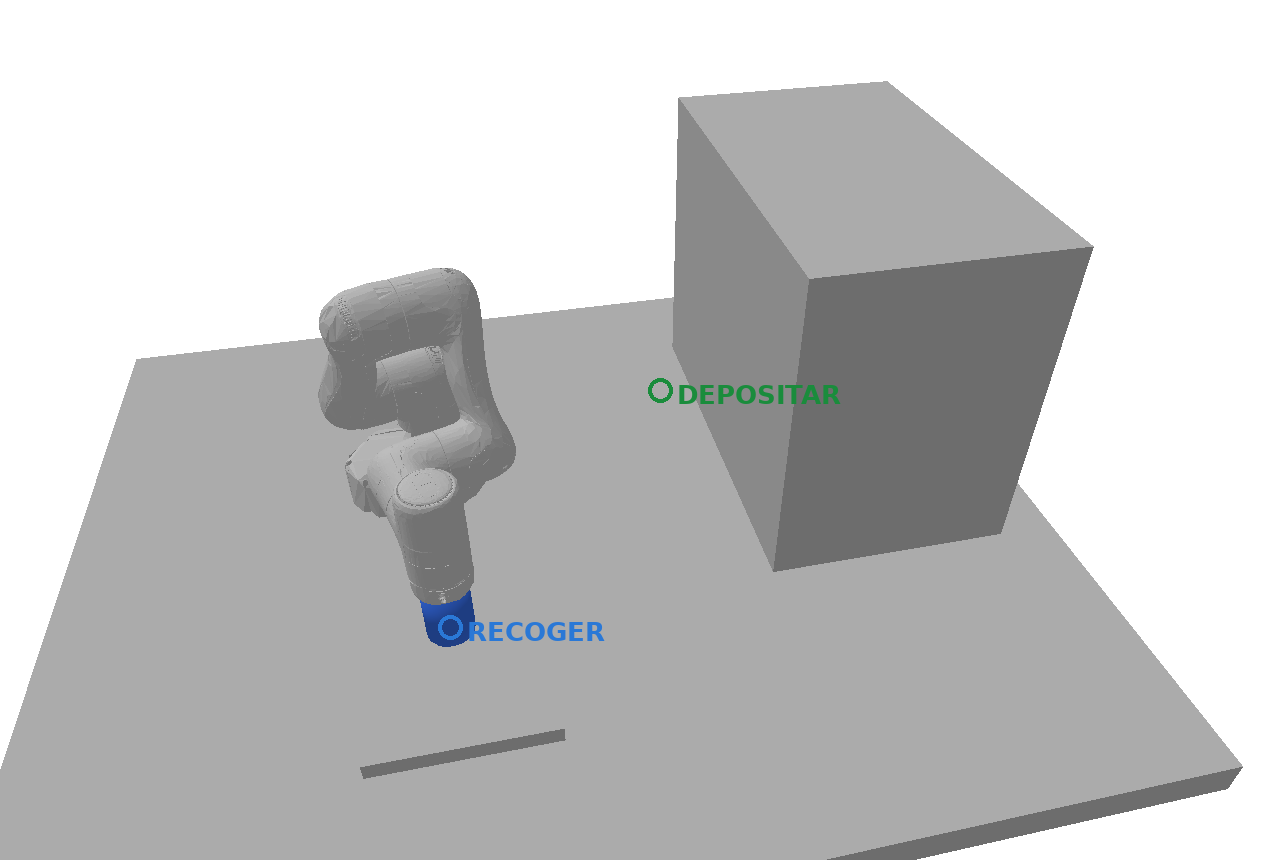
\includegraphics[width=\textwidth]{img/escena_1.png}\caption{Escenario 1: espacio libre}\end{subfigure}\hfill
\begin{subfigure}{0.48\textwidth}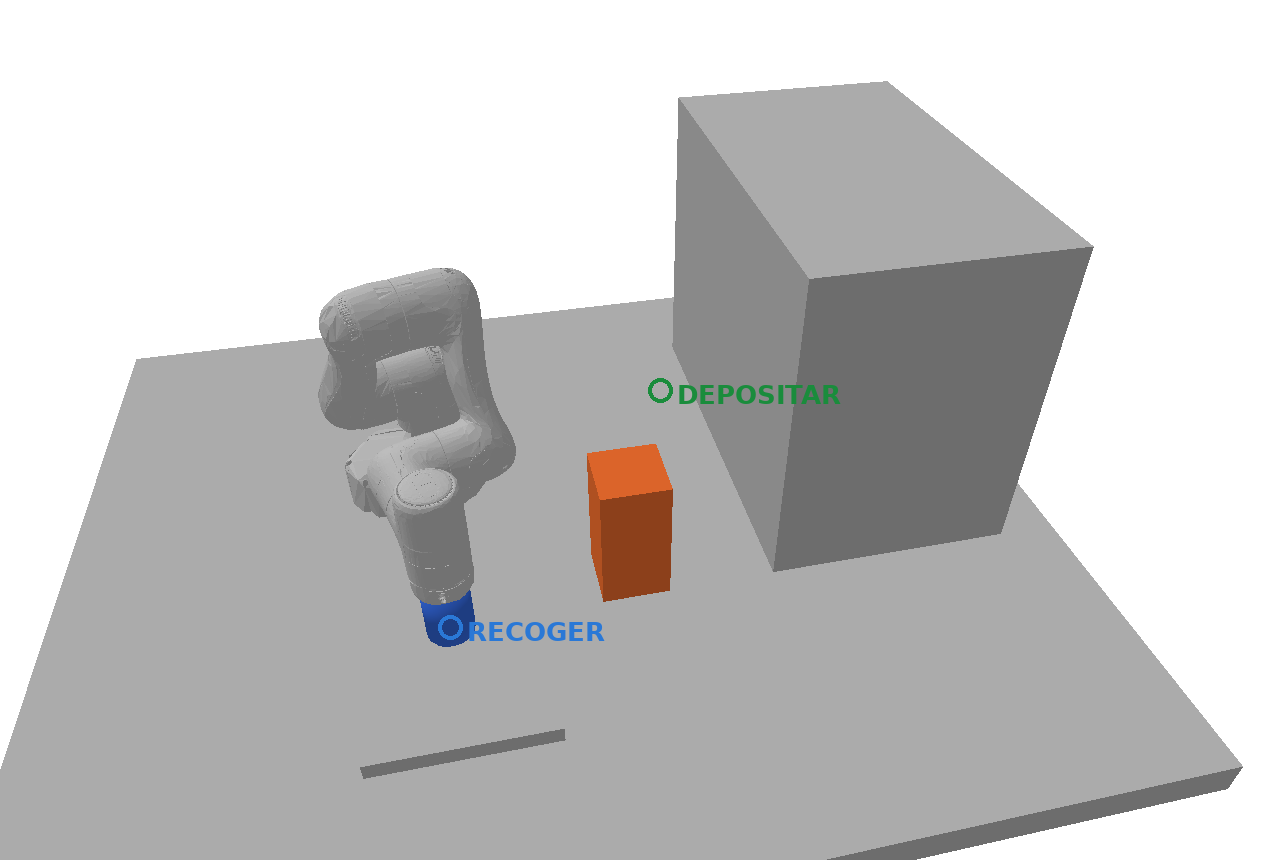
\includegraphics[width=\textwidth]{img/escena_2.png}\caption{Escenario 2: obstáculo único}\end{subfigure}\\[4pt]
\begin{subfigure}{0.48\textwidth}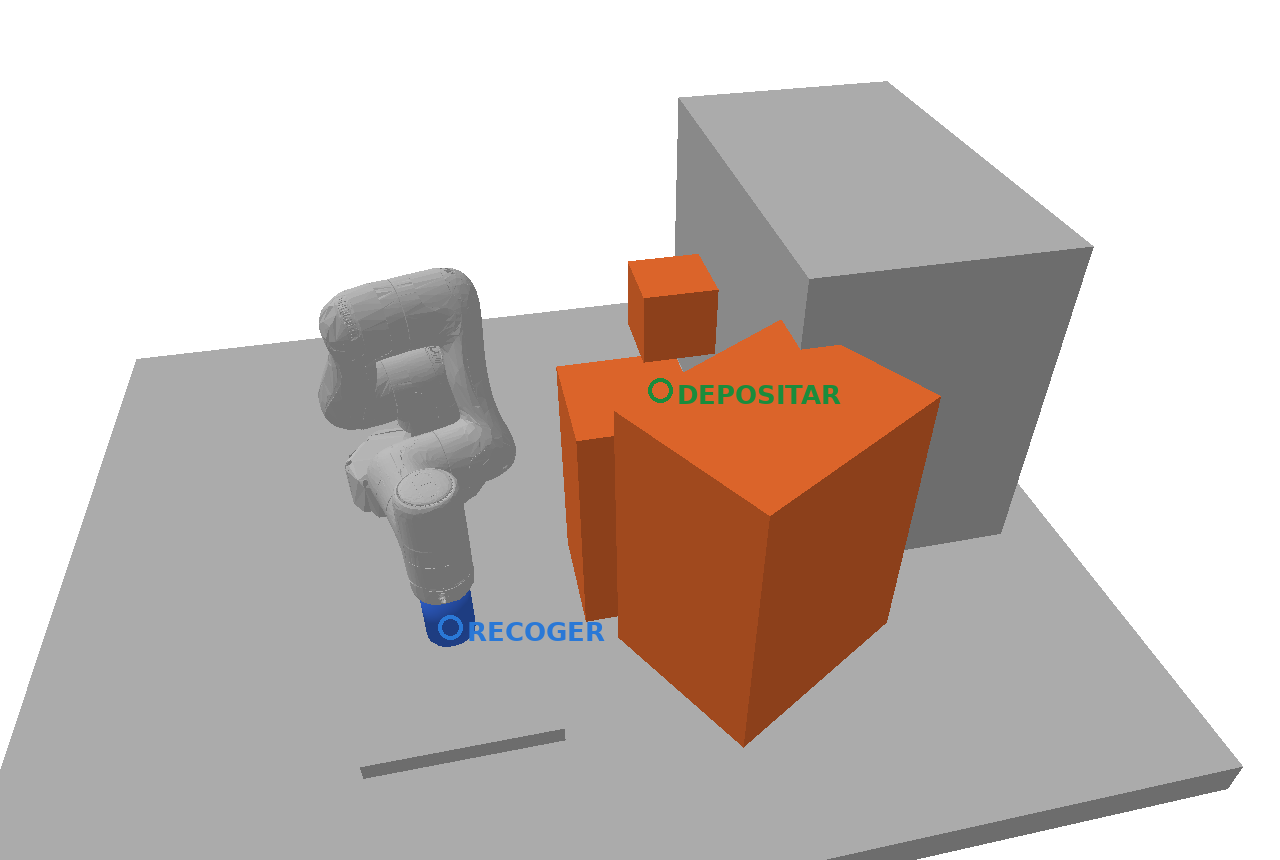
\includegraphics[width=\textwidth]{img/escena_3.png}\caption{Escenario 3: tres obstáculos}\end{subfigure}\hfill
\begin{subfigure}{0.48\textwidth}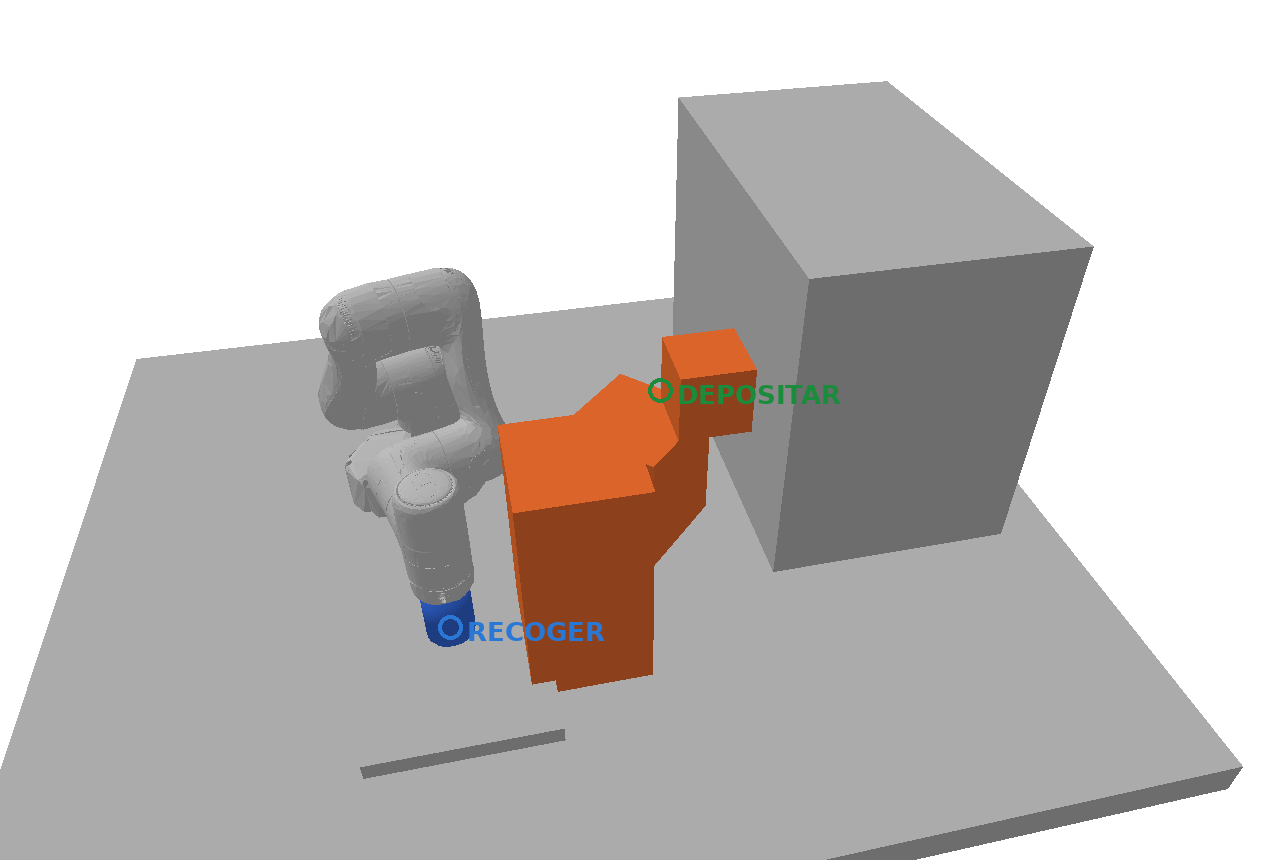
\includegraphics[width=\textwidth]{img/escena_8.png}\caption{Escenario 8: utillaje no visto}\end{subfigure}
\caption{Escenas del simulador. El círculo azul marca la recogida y el verde, el depósito.}
\end{figure}

\subsubsection{Resultados frente a la línea base}

La línea base fue evaluada con RRT-Connect en 296 de 300 intentos (98.7\,\%) y con LazyPRM* en 99 de 100, sin colisiones. La política SAC con la selección de la mejor validación fue evaluada una sola vez en 100 escenas fijas, con tres semillas independientes entrenadas $10^6$ pasos.

\begin{table}[H]
\centering
\caption{Resultados en 100 escenas de evaluación}
\small
\begin{tabular}{@{}lccc@{}}
\toprule
\textbf{Método} & \textbf{Éxito} & \textbf{Cómputo (ms)} & \textbf{Holgura mín. (mm)} \\
\midrule
RRT-Connect & 0.987 & 97.8 & 4 \\
LazyPRM* & 0.990 & 5\,043 & --- \\
SAC semilla 0 & 0.68 & \multirow{3}{*}{19.4 (media)} & \multirow{3}{*}{30 (media)} \\
SAC semilla 1 & 0.43 & & \\
SAC semilla 2 & 0.87 & & \\
\textbf{SAC, media de 3 semillas} & \textbf{0.66} & & \\
\bottomrule
\end{tabular}
\end{table}

\begin{figure}[H]
\centering
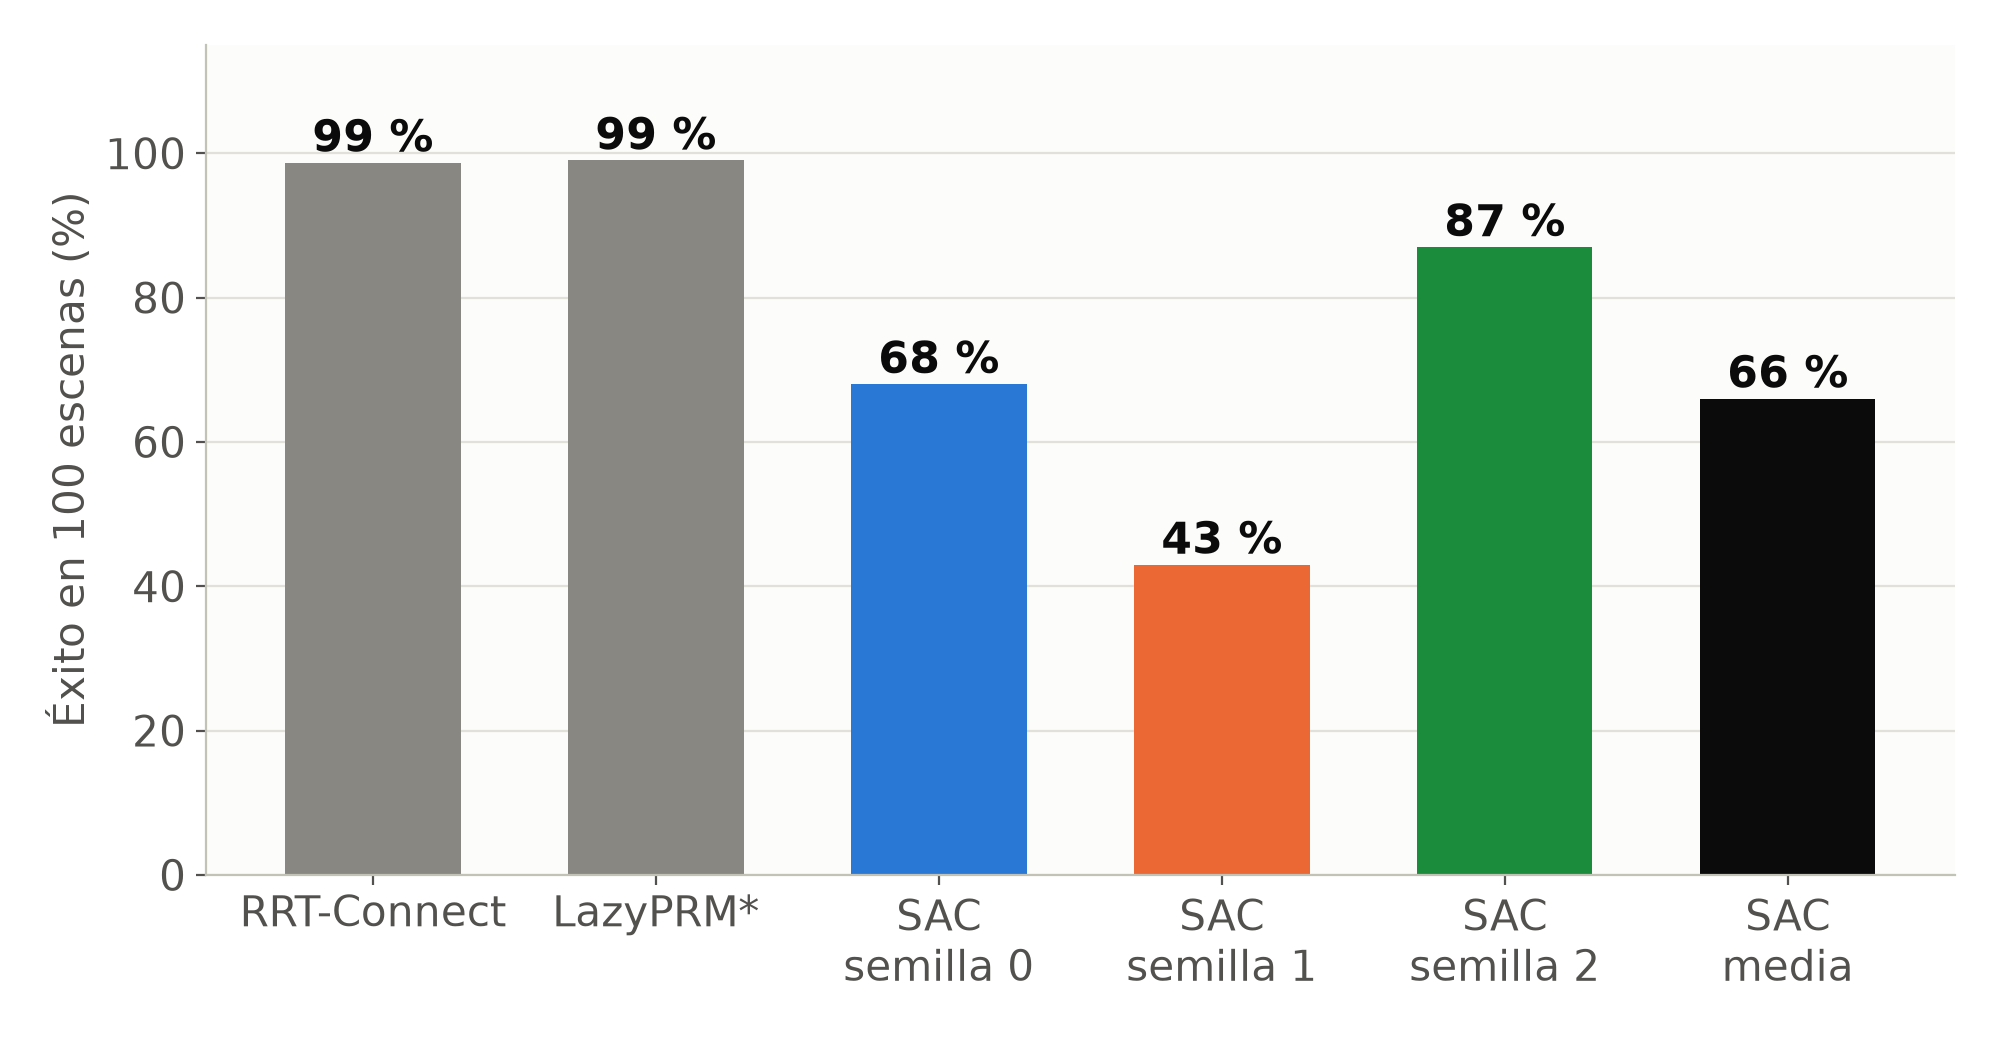
\includegraphics[width=0.78\textwidth]{img/fig_exito.png}
\caption{Tasa de éxito en 100 escenas: planificadores clásicos y tres semillas de SAC.}
\end{figure}

La comparación pareada de la política (tres semillas) con RRT-Connect, mediante la prueba de Wilcoxon, arroja:
\begin{itemize}
\item \textbf{Éxito}: 0.667 frente a 1.000; la línea base es mejor ($p=5\times10^{-11}$).
\item \textbf{Cómputo}: 19.4\,ms por episodio frente a 97.8\,ms; la política es mejor.
\item \textbf{Holgura mínima a obstáculos}: 30\,mm frente a 4\,mm; la política es mejor.
\item \textbf{Tiempo de ejecución} ($p=0.87$) y \textbf{longitud cartesiana}: sin diferencia significativa; la longitud articular es menor en la línea base.
\end{itemize}
La política tuvo colisión en el 2\,\% de los episodios. Con un episodio de unos 2\,s ($\approx$68 pasos), 19.4\,ms de inferencia equivalen a unos 0.3\,ms por paso, muy por debajo del período de control de 30\,ms.

\subsubsection{Dónde falla y cómo generaliza}

El éxito cae al crecer el obstáculo: con la semilla 2 pasa de 1.00 en los obstáculos más pequeños a 0.62 en los más grandes, y con las semillas 0 y 1 cae de 0.86 a 0.38 y de 0.62 a 0.19. Casi todos los fallos son tiempo agotado a 3--7\,cm de la meta; entre el 4 y el 15\,\% terminan en colisión. Entre las 19 variantes del contrato, las semillas aciertan 0.63, 0.42 y 0.84. En los escenarios fuera de distribución (3 y 8) el éxito es 0\,\% y en el paso estrecho (7), entre 0 y 67\,\%. Ese es precisamente el régimen en que el planificador clásico sigue siendo necesario.

\begin{figure}[H]
\centering
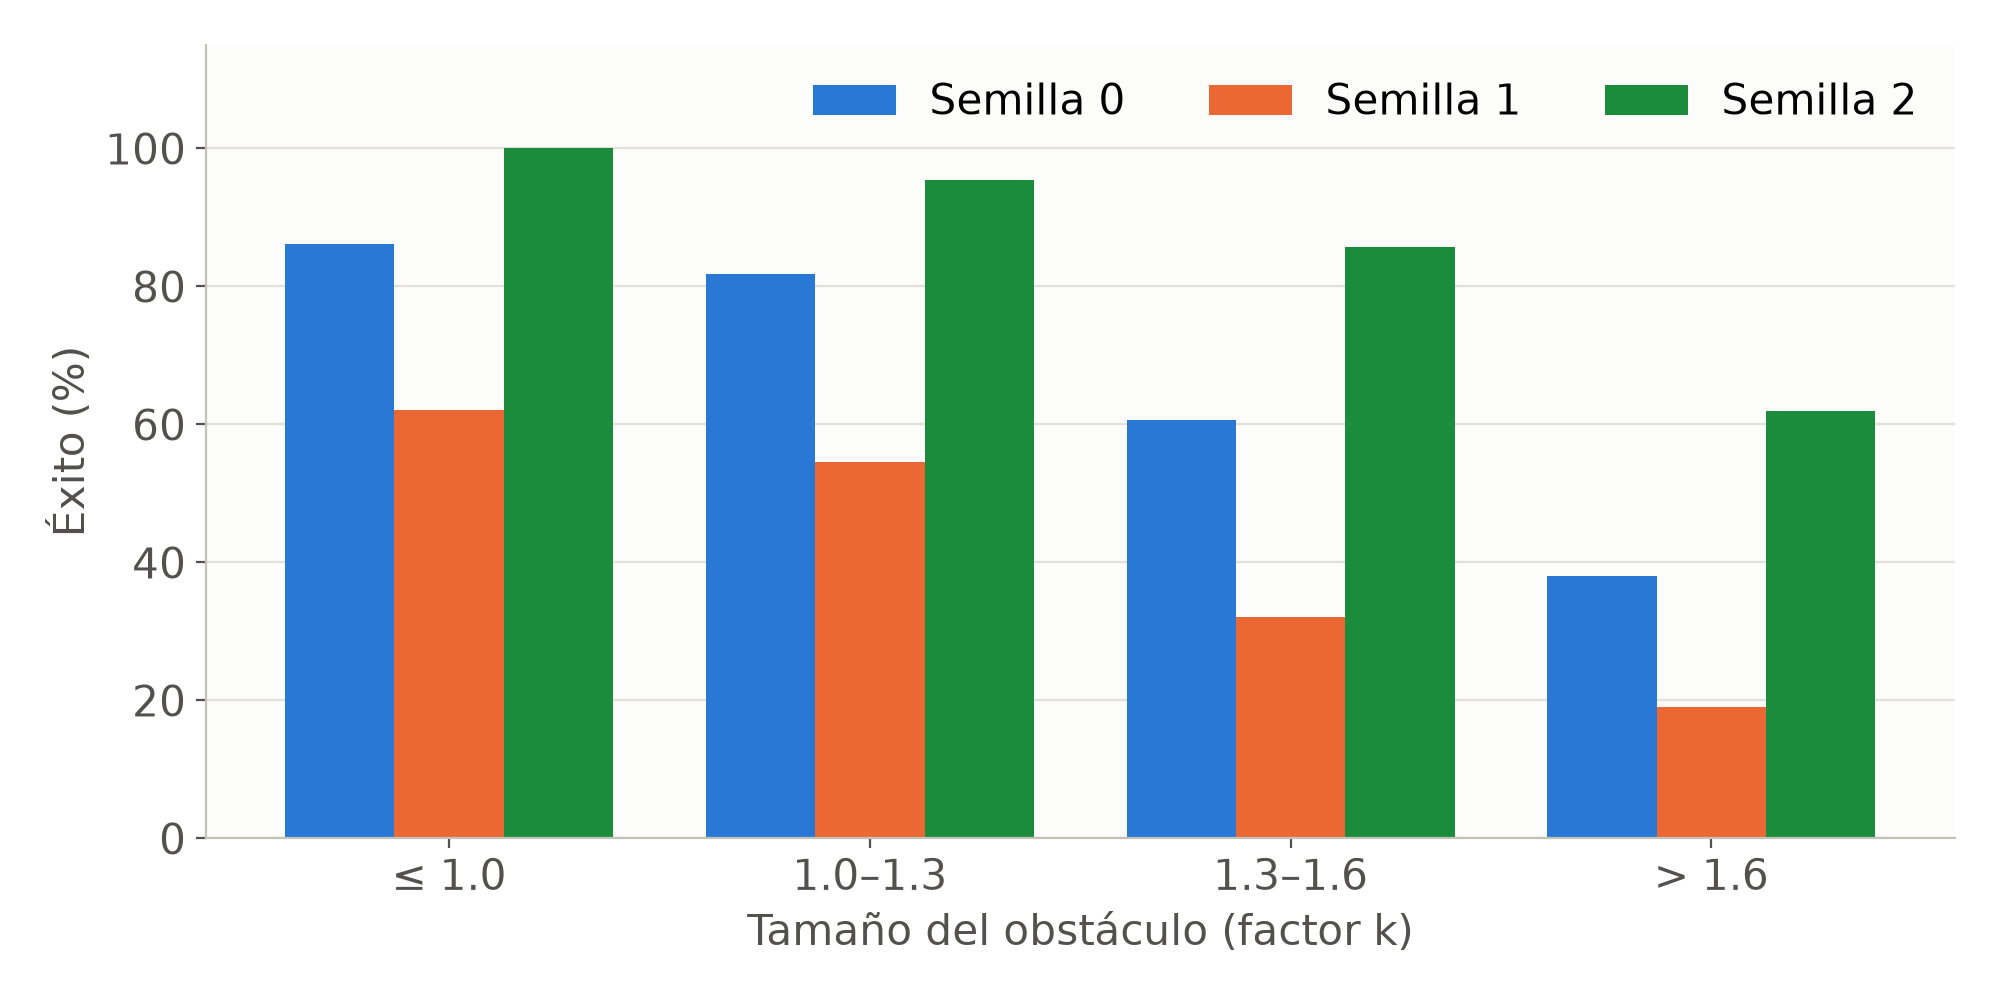
\includegraphics[width=0.8\textwidth]{img/fig_tamano.png}
\caption{Éxito por tamaño del obstáculo ($k$) para las tres semillas.}
\end{figure}

\subsubsection{Problemas encontrados y soluciones}

\begin{itemize}
\item \textbf{Modelo del E6 poco realista}: masas de 0.94\,kg en lugar de 7.2\,kg, límites rellenos y mallas de colisión huecas. Se generó un modelo corregido (\texttt{gen\_modelo\_e6.py}) como fuente única para los tres motores.
\item \textbf{Currículo que no llegaba a los entornos}: la primera implementación fijaba el atributo en el envoltorio de Stable-Baselines3 y no en el entorno. Una prueba lo detectó antes de entrenar; se cambió a un método reenviado por \texttt{env\_method}.
\item \textbf{La GPU no aceleraba el entrenamiento en el portátil}: la red es pequeña y domina la latencia de lanzar núcleos CUDA. Se pasó a la PC de 8 núcleos con GPU y cuatro corridas en paralelo (unas 3 h 45 min por corrida).
\item \textbf{GPU antigua}: la GTX 1080 (sm\_61) no es compatible con PyTorch cu130; se usó la variante cu126.
\item \textbf{Variabilidad entre semillas}: el éxito varía de 0.43 a 0.87 con el mismo algoritmo, por lo que se reportan siempre las tres semillas y no solo la mejor.
\end{itemize}

\section{Conclusiones y comentarios finales}

\begin{enumerate}
\item El problema de reconfiguración de celdas es real y está poco cubierto en el Perú, y las soluciones comerciales dependen de licencias o de GPU. Un estudio con software abierto que mida cuándo basta una política aprendida es pertinente.
\item Ya se dispone de la infraestructura completa: modelo corregido del E6, entorno de simulación, línea base clásica, tres entrenamientos de $10^6$ pasos y un evaluador común con cinco métricas.
\item Con la formulación actual la política \emph{no} iguala a la línea base en éxito (0.66 de media frente a 0.99), y su resultado varía mucho entre semillas (0.43 a 0.87). Ofrece, en cambio, menos cómputo (19.4 frente a 97.8\,ms) y mayor holgura (30 frente a 4\,mm). Es una conclusión de este periodo, no de conocimiento general.
\item La política falla sobre todo con obstáculos grandes y fuera de la distribución de entrenamiento. Las siguientes iteraciones se concentran en el muestreo de entrenamiento (más peso a obstáculos grandes y a escenas más variadas) y en la recompensa, y en validar con más escenas para no sobreajustar la selección del modelo.
\item Quedan por hacer el diseño electrónico de la integración con el E6, el análisis estadístico final y la demostración en vivo.
\end{enumerate}

\section{Referencias bibliográficas}
\makeatletter\let\origsection\section\def\section{\@ifstar\@gobble\origsection}\makeatother
\begin{thebibliography}{99}
\small
\bibitem{mao2025} J. L. Mao, Z. Wang, X. Zhou, F. Xia y C. L. Zhang, <<Design and experimental verification of a dynamic obstacle avoidance algorithm for robot manipulators based on deep reinforcement learning>> (en chino, resumen en inglés), \emph{Experimental Technology and Management}, vol. 42, n.º 4, pp. 78--85, abr. 2025, doi: 10.16791/j.cnki.sjg.2025.04.010.
\bibitem{fu2025} T. Fu y X. Tang, <<Optimizing robotic arm obstacle avoidance via improved random tree star (RRT)* and deep reinforcement learning coordination>>, \emph{Symmetry}, vol. 17, n.º 12, art. 2112, dic. 2025, doi: 10.3390/sym17122112.
\bibitem{xia2024} W. Xia, Y. Lu, W. Xu y X. Xu, <<Deep reinforcement learning based proactive dynamic obstacle avoidance for safe human-robot collaboration>>, \emph{Manufacturing Letters}, vol. 41, pp. 1246--1256, oct. 2024, doi: 10.1016/j.mfglet.2024.09.151.
\bibitem{fidalgo2025} I. Fidalgo Astorquia, G. Villate-Castillo, A. Tellaeche y J.-I. Vazquez, <<Comparative benchmark of sampling-based and DRL motion planning methods for industrial robotic arms>>, \emph{Sensors}, vol. 25, n.º 17, art. 5282, ago. 2025, doi: 10.3390/s25175282.
\bibitem{jurgenson2019} T. Jurgenson y A. Tamar, <<Harnessing reinforcement learning for neural motion planning>>, en \emph{Proc. Robotics: Science and Systems (RSS)}, 2019, arXiv:1906.00214.
\bibitem{liu2024} J. Liu, <<Geometric fabrics guided learning for collision-free manipulator global motion generation>>, tesis de B.A.Sc., Div. of Engineering Science, University of Toronto, Toronto, Canadá, 2024.
\bibitem{sanches2021} F. P. Sanches, <<End-to-end visual obstacle avoidance for a robotic manipulator using deep reinforcement learning>>, disertación de maestría, ICMC, Universidade de São Paulo, São Carlos, Brasil, 2021, doi: 10.11606/D.55.2021.tde-30082021-100712.
\bibitem{fidalgotesis} I. Fidalgo Astorquia, <<Estudio de la planificación de trayectorias en entornos dinámicos para manipuladores industriales mediante aprendizaje por refuerzo>>, tesis doctoral, Universidad de Deusto, Bilbao, España, 2025.
\bibitem{rapidplan} Realtime Robotics, <<RapidPlan>>. Accedido: 19 sep. 2026. [En línea]. Disponible: https://rtr.ai/rapidplan/
\bibitem{cumotion} NVIDIA Corporation, <<Making industrial robots more nimble with NVIDIA Isaac Manipulator and Vention MachineMotion AI>>, \emph{NVIDIA Developer Blog}. Accedido: 19 sep. 2026. [En línea]. Disponible: https://developer.nvidia.com/blog/making-industrial-robots-more-nimble-with-nvidia-isaac-manipulator-and-vention-machinemotion-ai
\bibitem{robodk} RoboDK Inc., <<Collision-free motion planner>>, \emph{RoboDK Documentation}. Accedido: 19 sep. 2026. [En línea]. Disponible: https://robodk.com/doc/en/Collision-Avoidance-Collision-Free-Motion-Planner.html
\bibitem{wang2023} C. Wang, H.-C. Lin y T. Kato, <<Collision avoidance motion planning method for industrial robot>>, U.S. Patente 11\,813\,753 B2, nov. 14, 2023.
\bibitem{levine2025} S. Levine, E. Holly, S. Gu y T. Lillicrap, <<Deep reinforcement learning for robotic manipulation>>, U.S. Patente 12\,240\,113 B2, mar. 4, 2025.
\bibitem{ifr2025} International Federation of Robotics, <<World Robotics 2025 report: industrial robots>>, comunicado de prensa, Frankfurt, 2025. Accedido: oct. 2026. [En línea]. Disponible: https://ifr.org/ifr-press-releases/news/global-robot-demand-in-factories-doubles-over-10-years
\bibitem{produce2025} Ministerio de la Producción (PRODUCE), OGEIEE, <<Estudio de investigación del sector metalmecánico 2024>>, citado en <<Sector metalmecánico genera 350 mil empleos y 74 mil empresas>>, \emph{ProActivo}, 16 jul. 2025. [En línea]. Disponible: https://proactivo.com.pe/sector-metalmecanico-genera-350-mil-empleos-y-74-mil-empresas/
\bibitem{aduana2019} Aduana News, <<Robots en América Latina: cuántos son, dónde están y cuánto tributan>>, cifras de la IFR. Accedido: oct. 2026. [En línea]. Disponible: https://aduananews.com/en/robots-en-america-latina-cuantos-son-donde-estan-y-cuanto-tributan/
\bibitem{fabricator} \emph{The Fabricator}, <<How robots program themselves>>. Accedido: oct. 2026. [En línea]. Disponible: https://www.thefabricator.com/thefabricator/article/automationrobotics/how-robots-program-themselves
\bibitem{e6precio} RobotLAB, <<DOBOT Magician E6>>, ficha de producto. Accedido: oct. 2026. [En línea]. Disponible: https://www.robotlab.com/store/dobot-magician-e6/
\bibitem{contexto} C. Camargo y L. L. Tupac Vásquez, <<Documento de contexto consolidado del proyecto>>, repositorio del proyecto, \texttt{docs/contexto-proyecto-rl-manipulador-6gdl.md}, 2026 (precio educativo de RoboDK consultado en robodk.com/pricing, sep. 2026).
\bibitem{haarnoja2018} T. Haarnoja, A. Zhou, P. Abbeel y S. Levine, <<Soft actor-critic: off-policy maximum entropy deep reinforcement learning with a stochastic actor>>, en \emph{Proc. ICML}, 2018, pp. 1861--1870.
\bibitem{haarnoja2018b} T. Haarnoja \emph{et al.}, <<Soft actor-critic algorithms and applications>>, arXiv:1812.05905, 2018.
\bibitem{sb3} A. Raffin \emph{et al.}, <<Stable-Baselines3: reliable reinforcement learning implementations>>, \emph{J. Mach. Learn. Res.}, vol. 22, n.º 268, pp. 1--8, 2021.
\bibitem{sutton2018} R. S. Sutton y A. G. Barto, \emph{Reinforcement Learning: An Introduction}, 2.ª ed. Cambridge, MA, EE. UU.: MIT Press, 2018.
\bibitem{siciliano2009} B. Siciliano, L. Sciavicco, L. Villani y G. Oriolo, \emph{Robotics: Modelling, Planning and Control}. Londres, Reino Unido: Springer, 2009.
\bibitem{kuffner2000} J. J. Kuffner y S. M. LaValle, <<RRT-Connect: an efficient approach to single-query path planning>>, en \emph{Proc. IEEE ICRA}, 2000, pp. 995--1001.
\bibitem{bohlin2000} R. Bohlin y L. E. Kavraki, <<Path planning using lazy PRM>>, en \emph{Proc. IEEE ICRA}, 2000, pp. 521--528.
\bibitem{karaman2011} S. Karaman y E. Frazzoli, <<Sampling-based algorithms for optimal motion planning>>, \emph{Int. J. Robotics Research}, vol. 30, n.º 7, pp. 846--894, 2011.
\bibitem{ompl} I. A. \c{S}ucan, M. Moll y L. E. Kavraki, <<The Open Motion Planning Library>>, \emph{IEEE Robotics \& Automation Magazine}, vol. 19, n.º 4, pp. 72--82, dic. 2012.
\bibitem{moveit} D. Coleman, I. \c{S}ucan, S. Chitta y N. Correll, <<Reducing the barrier to entry of complex robotic software: a MoveIt! case study>>, \emph{J. Software Engineering for Robotics}, vol. 5, n.º 1, pp. 3--16, 2014.
\bibitem{fcl} J. Pan, S. Chitta y D. Manocha, <<FCL: a general purpose library for collision and proximity queries>>, en \emph{Proc. IEEE ICRA}, 2012, pp. 3859--3866.
\bibitem{wilcoxon1945} F. Wilcoxon, <<Individual comparisons by ranking methods>>, \emph{Biometrics Bulletin}, vol. 1, n.º 6, pp. 80--83, 1945.
\end{thebibliography}

\end{document}
